% Created by tikzDevice version 0.10.1 on 2016-07-28 16:07:26
% !TEX encoding = UTF-8 Unicode
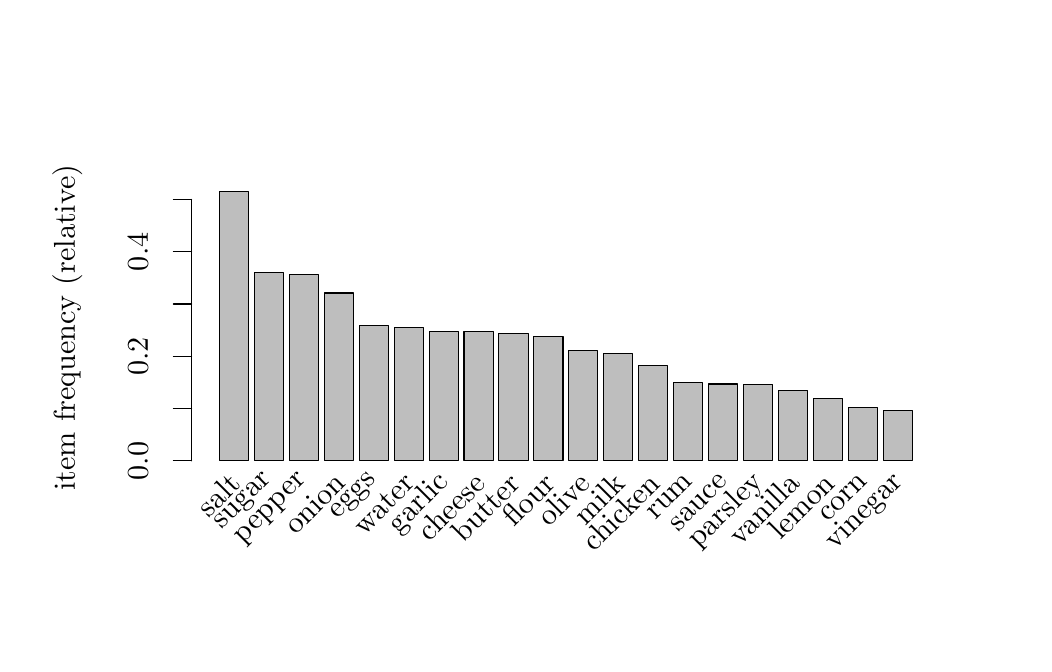
\begin{tikzpicture}[x=1pt,y=1pt]
\definecolor{fillColor}{RGB}{255,255,255}
\path[use as bounding box,fill=fillColor,fill opacity=0.00] (0,0) rectangle (360.07,222.54);
\begin{scope}
\path[clip] (  0.00,  0.00) rectangle (360.07,222.54);
\definecolor{drawColor}{RGB}{0,0,0}
\definecolor{fillColor}{RGB}{190,190,190}

\path[draw=drawColor,line width= 0.4pt,line join=round,line cap=round,fill=fillColor] ( 69.28, 65.99) rectangle ( 79.80,163.28);

\path[draw=drawColor,line width= 0.4pt,line join=round,line cap=round,fill=fillColor] ( 81.90, 65.99) rectangle ( 92.43,134.21);

\path[draw=drawColor,line width= 0.4pt,line join=round,line cap=round,fill=fillColor] ( 94.53, 65.99) rectangle (105.05,133.46);

\path[draw=drawColor,line width= 0.4pt,line join=round,line cap=round,fill=fillColor] (107.16, 65.99) rectangle (117.68,126.65);

\path[draw=drawColor,line width= 0.4pt,line join=round,line cap=round,fill=fillColor] (119.78, 65.99) rectangle (130.31,115.01);

\path[draw=drawColor,line width= 0.4pt,line join=round,line cap=round,fill=fillColor] (132.41, 65.99) rectangle (142.93,114.23);

\path[draw=drawColor,line width= 0.4pt,line join=round,line cap=round,fill=fillColor] (145.04, 65.99) rectangle (155.56,112.62);

\path[draw=drawColor,line width= 0.4pt,line join=round,line cap=round,fill=fillColor] (157.66, 65.99) rectangle (168.18,112.61);

\path[draw=drawColor,line width= 0.4pt,line join=round,line cap=round,fill=fillColor] (170.29, 65.99) rectangle (180.81,112.09);

\path[draw=drawColor,line width= 0.4pt,line join=round,line cap=round,fill=fillColor] (182.92, 65.99) rectangle (193.44,110.97);

\path[draw=drawColor,line width= 0.4pt,line join=round,line cap=round,fill=fillColor] (195.54, 65.99) rectangle (206.06,105.87);

\path[draw=drawColor,line width= 0.4pt,line join=round,line cap=round,fill=fillColor] (208.17, 65.99) rectangle (218.69,104.75);

\path[draw=drawColor,line width= 0.4pt,line join=round,line cap=round,fill=fillColor] (220.79, 65.99) rectangle (231.32,100.32);

\path[draw=drawColor,line width= 0.4pt,line join=round,line cap=round,fill=fillColor] (233.42, 65.99) rectangle (243.94, 94.22);

\path[draw=drawColor,line width= 0.4pt,line join=round,line cap=round,fill=fillColor] (246.05, 65.99) rectangle (256.57, 93.78);

\path[draw=drawColor,line width= 0.4pt,line join=round,line cap=round,fill=fillColor] (258.67, 65.99) rectangle (269.20, 93.64);

\path[draw=drawColor,line width= 0.4pt,line join=round,line cap=round,fill=fillColor] (271.30, 65.99) rectangle (281.82, 91.55);

\path[draw=drawColor,line width= 0.4pt,line join=round,line cap=round,fill=fillColor] (283.93, 65.99) rectangle (294.45, 88.70);

\path[draw=drawColor,line width= 0.4pt,line join=round,line cap=round,fill=fillColor] (296.55, 65.99) rectangle (307.07, 85.26);

\path[draw=drawColor,line width= 0.4pt,line join=round,line cap=round,fill=fillColor] (309.18, 65.99) rectangle (319.70, 84.31);

\node[text=drawColor,rotate= 90.00,anchor=base,inner sep=0pt, outer sep=0pt, scale=  1.09] at ( 17.02,114.15) {item frequency (relative)};
\end{scope}
\begin{scope}
\path[clip] (  0.00,  0.00) rectangle (360.07,222.54);
\definecolor{drawColor}{RGB}{0,0,0}

\path[draw=drawColor,line width= 0.4pt,line join=round,line cap=round] ( 59.26, 65.99) -- ( 59.26,160.46);

\path[draw=drawColor,line width= 0.4pt,line join=round,line cap=round] ( 59.26, 65.99) -- ( 52.66, 65.99);

\path[draw=drawColor,line width= 0.4pt,line join=round,line cap=round] ( 59.26, 84.88) -- ( 52.66, 84.88);

\path[draw=drawColor,line width= 0.4pt,line join=round,line cap=round] ( 59.26,103.78) -- ( 52.66,103.78);

\path[draw=drawColor,line width= 0.4pt,line join=round,line cap=round] ( 59.26,122.67) -- ( 52.66,122.67);

\path[draw=drawColor,line width= 0.4pt,line join=round,line cap=round] ( 59.26,141.57) -- ( 52.66,141.57);

\path[draw=drawColor,line width= 0.4pt,line join=round,line cap=round] ( 59.26,160.46) -- ( 52.66,160.46);

\node[text=drawColor,rotate= 90.00,anchor=base,inner sep=0pt, outer sep=0pt, scale=  1.09] at ( 43.42, 65.99) {0.0};

\node[text=drawColor,rotate= 90.00,anchor=base,inner sep=0pt, outer sep=0pt, scale=  1.09] at ( 43.42,103.78) {0.2};

\node[text=drawColor,rotate= 90.00,anchor=base,inner sep=0pt, outer sep=0pt, scale=  1.09] at ( 43.42,141.57) {0.4};
\end{scope}
\begin{scope}
\path[clip] (  0.00,  0.00) rectangle (360.07,222.54);
\definecolor{drawColor}{RGB}{0,0,0}

\node[text=drawColor,rotate= 45.00,anchor=base east,inner sep=0pt, outer sep=0pt, scale=  1.09] at ( 77.45, 57.19) {salt};

\node[text=drawColor,rotate= 45.00,anchor=base east,inner sep=0pt, outer sep=0pt, scale=  1.09] at ( 88.16, 59.10) {sugar};

\node[text=drawColor,rotate= 45.00,anchor=base east,inner sep=0pt, outer sep=0pt, scale=  1.09] at (100.79, 59.10) {pepper};

\node[text=drawColor,rotate= 45.00,anchor=base east,inner sep=0pt, outer sep=0pt, scale=  1.09] at (115.23, 57.29) {onion};

\node[text=drawColor,rotate= 45.00,anchor=base east,inner sep=0pt, outer sep=0pt, scale=  1.09] at (126.04, 59.10) {eggs};

\node[text=drawColor,rotate= 45.00,anchor=base east,inner sep=0pt, outer sep=0pt, scale=  1.09] at (140.27, 57.50) {water};

\node[text=drawColor,rotate= 45.00,anchor=base east,inner sep=0pt, outer sep=0pt, scale=  1.09] at (152.39, 58.01) {garlic};

\node[text=drawColor,rotate= 45.00,anchor=base east,inner sep=0pt, outer sep=0pt, scale=  1.09] at (165.83, 57.19) {cheese};

\node[text=drawColor,rotate= 45.00,anchor=base east,inner sep=0pt, outer sep=0pt, scale=  1.09] at (178.46, 57.19) {butter};

\node[text=drawColor,rotate= 45.00,anchor=base east,inner sep=0pt, outer sep=0pt, scale=  1.09] at (191.09, 57.19) {flour};

\node[text=drawColor,rotate= 45.00,anchor=base east,inner sep=0pt, outer sep=0pt, scale=  1.09] at (203.71, 57.19) {olive};

\node[text=drawColor,rotate= 45.00,anchor=base east,inner sep=0pt, outer sep=0pt, scale=  1.09] at (216.34, 57.19) {milk};

\node[text=drawColor,rotate= 45.00,anchor=base east,inner sep=0pt, outer sep=0pt, scale=  1.09] at (228.96, 57.19) {chicken};

\node[text=drawColor,rotate= 45.00,anchor=base east,inner sep=0pt, outer sep=0pt, scale=  1.09] at (240.50, 58.28) {rum};

\node[text=drawColor,rotate= 45.00,anchor=base east,inner sep=0pt, outer sep=0pt, scale=  1.09] at (253.13, 58.28) {sauce};

\node[text=drawColor,rotate= 45.00,anchor=base east,inner sep=0pt, outer sep=0pt, scale=  1.09] at (266.02, 58.01) {parsley};

\node[text=drawColor,rotate= 45.00,anchor=base east,inner sep=0pt, outer sep=0pt, scale=  1.09] at (279.47, 57.19) {vanilla};

\node[text=drawColor,rotate= 45.00,anchor=base east,inner sep=0pt, outer sep=0pt, scale=  1.09] at (292.10, 57.19) {lemon};

\node[text=drawColor,rotate= 45.00,anchor=base east,inner sep=0pt, outer sep=0pt, scale=  1.09] at (303.63, 58.28) {corn};

\node[text=drawColor,rotate= 45.00,anchor=base east,inner sep=0pt, outer sep=0pt, scale=  1.09] at (316.43, 58.11) {vinegar};
\end{scope}
\end{tikzpicture}
